\documentclass{article}
\usepackage[utf8]{inputenc}
\usepackage{listings}
\usepackage{color}
\usepackage{tikz}
\usetikzlibrary{shapes}
\usepackage{graphicx}
\graphicspath{ {images/} }
\usepackage{hyperref}

\definecolor{dkgreen}{rgb}{0,0.6,0}
\definecolor{gray}{rgb}{0.5,0.5,0.5}
\definecolor{mauve}{rgb}{0.58,0,0.82}

\lstset{frame=tb,
  language=C,
  aboveskip=3mm,
  belowskip=3mm,
  showstringspaces=false,
  columns=flexible,
  basicstyle={\small\ttfamily},
  numbers=none,
  numberstyle=\tiny\color{gray},
  keywordstyle=\color{blue},
  commentstyle=\color{dkgreen},
  stringstyle=\color{mauve},
  breaklines=true,
  breakatwhitespace=true,
  tabsize=3
}

\begin{document}

\title{Relatório Fase III}
\author{André Camargo Perello - 9912403\\Lucas Henrique Bahr Yau - 9763832\\Rudá Lima da Floresta  9912410}
\date{}

\maketitle
\newpage
    \section{Introdução}
    Nesta fase tivemos de enriquecer o código feito na fase anterior e fazer a comunicação entre o código em $\mathcal{C}$ e a representação gráfica do jogo feita com o pacote $pygame$ do $Python$. Dessa forma, dentre os principais objetivos desta fase estão:
    \begin{itemize}
        \item Inserir os exércitos próximos às bases
        \item Representar graficamente os robôs e seus movimentos
        \item Representar graficamente os tipos de terreno
        \item Representar graficamente os cristais
        \item Enriquecer a ação ATTK
    \end{itemize}

    Todos os sprites utilizados foram obtidos do site \href{opengameart.org}{OpenGameArt}. Os objetivos pedidos na especificação que não estão listados aqui já foram implementados na fase anterior. Nas seções seguintes do relatório explicaremos como as novas funcionalidades foram implementadas e os problemas que encontramos no caminho. Além disso, todos os testes anteriormente feitos agora também servem para testar a interface gráfica.
    
    
    \section{Exércitos e Bases}
    Antes de falar sobre as bases e os exércitos, encontramos um problema na representação gráfica da nossa matriz. O código fornecido no arquivo $apres$ cria a arena com células hexagonais, porém mantém a implementação de uma matriz quadrada, ignorando as vizinhanças que são possíveis caso fosse uma matriz que imitasse um grid hexagonal. Dessa forma, toda vez que passamos índices da matriz para o $apres$, mudamos o índice para que ele se adapte à implementação. De fato, encontramos uma transformação que adapta os índices, porém tivemos de, ao criar o grid, criar uma matriz retangular $\mathcal{M}_{n\times2n}$,, logo sempre que á um índice válido na matriz original $(i, j)$ equivale ao índice $(i, j/2)$ na matriz do $apres$, onde a divisão é inteira.
    
    Além disso, foi dito na especificação que um robô básico teria, dentre outras coisas, um objeto para guardar a vizinhança apresentada pelo sistema. Porém, assim como documentado no relatório anterior, para que o robô "enxergue" em uma determinada direção, ele deve solicitar essa ação. Dessa forma, adicionar um objeto desse tipo ao robô mudaria completamente nossa implementação, dissiparia parte da complexidade do jogo e implicitamente daria ao robô acesso à arena, o que não faria sentido considerando as fases anteriores.
    
    As bases foram postas nos cantos superior esquerdo e inferior direito da tela por simplificação da implementação. Além disso, optamos por inserir os exércitos em fileira próximos à base. Embora a ideia inicial tenha sido colocar os robôs aleatoriamente, encontramos diversas dificuldades com a implementação. A imagem a seguir ilustra uma arena básica de tamanho 7x7 com 5 robôs em cada exército. 
    
    \begin{figure}[h]
        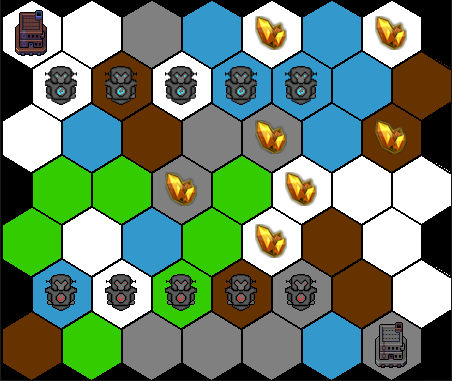
\includegraphics[width=8cm]{7x7.png}
        \centering
    \end{figure}
    
    Para esta fase, adicionamos à struct Maquina novos objetos, de modo que ela se encontra da forma:
    
    \begin{lstlisting}
    typedef struct {  
    	Pilha pil;
    	Pilha exec;
    	OPERANDO Mem[MAXMEM];
    	INSTR *prog;
    	int ip;
    	int rbp;
    	int x;
    	int y;
    	int oldX;
    	int oldY;
    	int hp;
    	int damage;
    	int defense;
    	Cristais crystals;
    	Bool alive;
    	Time t;
    	int time;
    	int id;
    } Maquina;
    \end{lstlisting}
    Agora, a Maquina precisa armazenar: suas posições antigas, para que a movimentação seja feita; seus pontos de vida (hp), ataque e defesa para o combate; e seu id e tempo de espera que ele precisa para realizar uma ação e ser identificado na matriz.  
    
    
    
    
    \section{Movimentação}
    A base da movimentação já havia sido implementada na fase anterior, porém, omo especificado, cada tipo de terreno tem um tempo de espera associado para que a ação de movimento ocorra. Em suma, se há um tipo de terreno onde é mais complicado para o robô se movimentar, adicionados um delay à ação. Dessa forma, o robô espera ciclos de tempo de jogo para executar. Desse modo, bastou adicionar o seguinte pedaço de código à função que realiza a movimentação do robô:
    
    \begin{lstlisting}
    
        switch(arena->grid[i][j].t) {
		case ESTRADA:
			break;
		case RIO:
			m->time += 2;
			break;		
		case MONTANHA:
			m->time += 5;
			break;
		case LAMA:
			m->time += 4;
			break;
		case CAMPO: 
			m->time += 1;
			break;
	}

    \end{lstlisting}
    
    Além disso, fizemos a comunicação com a parte gráfica do jogo utilizando a função:
    \begin{lstlisting}
    void printRobot(Maquina* maq) {
    	int i, j;
    	i = maq->y;
    	j = maq->x / 2;
    	
    	fprintf(display, "%d %d %d %d %d\n",
    						maq->id, maq->oldY, maq->oldX / 2, i, j);
    	fflush(display);
    }

    \end{lstlisting}
    Esta função apenas adapta os valores da matriz original para a matriz do apres e envia o id da máquina, suas antigas e novas posições. Assim, o apres deleta o sprite na posição antiga e redesenha o robô na posição nova.
    
    \section{Terrenos}
    Decidimos por apenas colocar cores específicas para cada tipo de terrenos devido a dificuldades encontradas no posicionamento de sprites específicos para cada terreno. Quando o grid é inicializado, escrevemos no apres o seguinte código:
    
    \begin{lstlisting}
    // Indica para o apres inserir um terreno na linha j, coluna i/2 de tipo arena->grid[i][j].t
    fprintf(display, "terr %d %d %d\n", j, i / 2 , (int)arena->grid[i][j].t);
    \end{lstlisting}
    
    Quando o apres recebe este código pela entrada padrão, ele executa o seguinte pedaço de código para desenhar o grid da cor correspondente ao terreno:
    
    \begin{lstlisting}
    if r[0] == 'terr':
        i = int(r[1])
        j = int(r[2])
        terrain = r[3]
        
        if terrain == '0':
            arena[i].append(cell(i, j, (128, 128, 128))) # Estrada: cinza
            
        elif terrain == '1':
            arena[i].append(cell(i, j, (51, 153, 204))) # Rio: azul
            
        elif terrain == '2':
            arena[i].append(cell(i, j, (255, 255, 255))) # Montanha: cinza
            
        elif terrain == '3':
            arena[i].append(cell(i, j, (102, 51, 0))) # Lama: marrom
            
        elif terrain == '4':
            arena[i].append(cell(i, j, (51, 204, 0))) # Campo: verde
            
        continue
        
    \end{lstlisting}
    
    Assim ele constrói a matriz de células e, quando o jogo é iniciado, ele as desenha da cor especificada.
    
    \section{Cristais}
    Quando a arena é inicializada, inicia-se um loop para inserir cristais na arena. Optamos por colocar no máximo, dado uma matriz $\mathcal{M}_{n\times n}$, $\frac{n}{2}$ cristais aleatoriamente em tordo da arena.
    
    \begin{lstlisting}
    for(int i = 0; i <= ncols / 2;) {
		
		int r1 = rand() % nrows;
		int r2 = (rand() % ncols);
		
		//Decide se as coordenadas são válidas para a matriz
		if((r1 % 2 == 0 && r2 % 2 == 0) || (r1 % 2 == 1 && r2 % 2 == 1) && arena->grid[r1][r2].o.ocupado == False) {
			arena->grid[r1][r2].c = True;
			arena->grid[r1][r2].o.ocupado = True;
			fprintf(display, "crys ./sprites/crystal.png %d %d\n", r1 , r2 / 2);

			i++;
		}
	}
        
    \end{lstlisting}
    
    A parcela que corresponde a comunicação do local dos cristais com o apres é dada por:
    
    \begin{lstlisting}
        fprintf(display, "crys ./sprites/crystal.png %d %d\n", r1 , r2 / 2);
    \end{lstlisting}
    
    Quando imprimimos esta sequência no apres, ele apenas pega o spride e o desenha no local especificado.
    
    \section{Batalha entre robôs}
    Como falamos na seção sobre a Arena e Exércitos, para integrar os ataques e seus respectivos danos aos robôs tivemos de adaptar o código, inserindo uma identificação para cada robô ao próprio robô. Além disso, tivemos de inserir essa mesma identificação à célula que ele ocupa, inserindo na parcela Ocupacao que cada célula possui. Além disso, o robô agora possui pontos de vida, pontos de ataque e de defesa. 
    
    Quando um robô pede ao sistema para atacar em uma direção e há um inimigo naquela direção, executamos o código:
    
    \begin{lstlisting}
    
   int enemy = getEnemy(arena, i, j);
	int damage = getDamage(m);
	printf("EXTERMINATE!\n");
	arena->exercitos[enemy]->hp -= damage - arena->exercitos[enemy]->defense;
		
	if(arena->exercitos[enemy]->hp < 0){
		fprintf(display, "die %d %d\n", i, (j/2));
		arena->grid[i][j].o.ocupado = False;
		arena->grid[i][j].o.id = -1;
	}
    \end{lstlisting}
    
    Na posição onde foi solicitado o ataque há a identificação de que robô está lá. Assim, a função $getEnemy$ busca o índice, no vetor de robôs da arena, desse robô para que sua vida e pontos de defesa possam ser acessados. Logo, executamos com a função $getDamage$ o código:
    
    \begin{lstlisting}
    int getDamage(Maquina *m){
	srand(time(NULL));
	int damage = m->damage + rand()%10;
	    if(m->hp < 50 && m->hp > 20)
	    	damage = damage/2;
	    else if(m->hp< 20)
	    	damage = damage/3;
	    return damage;
    }

    \end{lstlisting}
    
    Essa função simplesmente pega o dano básico do robô e adiciona à um número aleatório $n \in [0\ldots9]$. Esse dano gerado aleatoriamente é diminuído de acordo com a vida do robô. Pretendemos sofisticar, na próxima fase, o modo como essa diminuição ocorre de acordo com os pontos de vida.
    
    Infelizmente, por falta de conhecimento, não conseguimos inserir uma animação para os ataques, porém pretendemos inserir isso na fase seguinte.
    
    \section{Dificuldades}
    
    Com certeza, a maior dificuldade nesta fase foi a implementação da visualização dos métodos pelo $apres$. O $pygame$ apenas aceita imagens de formato $*.png$ e não soubemos como retirar os sprites inseridos na tela sem ter que redesenhar algo por cima. Dessa forma, boa parte dos efeitos e ações que desejávamos inserir não foram colocadas. Além disso, as diferenças entre a implementação autoral e a implementação que nos foi fornecida, dificultou boa parte da fase. Tivemos de passar mais tempo tentando entender o código alheio e achar transformações entre os nossos índices e os índices usados no $apres$ que realmente implementando o que foi requisitado para esta fase.
    
    \section{Conclusão}
    Embora tivemos contratempos, esta fase se revelou mais simples que a fase anterior. Boa parte das funcionalidades já estavam implementadas, então bastaram algumas adaptações ao código para que tudo fluísse bem. 

\end{document}